\nonstopmode
\documentclass{beamer}
%\documentclass[handout]{beamer}
%\includeonlylecture{week12}



\providecommand{\cpp}{C\kern-0.05em\texttt{+\kern-0.03em+} }
\providecommand{\Cpp}{\cpp}

%\usepackage{pdfpages}
\usepackage[utf8]{inputenc}
\usepackage[T1]{fontenc}
\usepackage{lmodern}
\usepackage{import}
\graphicspath{{../pics}}
%\usepackage{pgf}
%\usepackage{ctable}

\usepackage{listings}%[2000/08/23]
\usepackage{lstlangampl} % syntax file, I added some more keywords like 'display'

%\usepackage{graphicx}
%\usepackage{multicol}

%\usepackage{tikz}

\lstnewenvironment{cplus}
    {\lstset{language=c++,basicstyle=\scriptsize,frame=}}
    {}


\lstnewenvironment{cplus3}
    {\lstset{language=c++,basicstyle=\scriptsize,frame=}}
    {}


\lstnewenvironment{java}
    {\lstset{language=java,basicstyle=\scriptsize,frame=}}
    {}

\lstnewenvironment{java2}
    {\lstset{language=java,basicstyle=\scriptsize}}
    {}

\lstdefinelanguage{Haskell-custom}
{%columns=flexible,
escapeinside={--@}{@--},breaklines=true,breakatwhitespace=true%
language=Haskell,basicstyle=\color{lightblue}\ttfamily,keywordstyle=\ttfamily,%
morekeywords={class,instance,type,newtype,data,where,deriving,import},%
lineskip=-.1\baselineskip,morekeywords={concept,requires,concept_map}}

\lstnewenvironment{hask}[1][\small]{\lstset{language=Haskell-custom,%
    style=numbers,basicstyle=\color{lightblue}#1\ttfamily,keywordstyle=#1\ttfamily,%
    style=bold-keywords,style=frametb}}{}

\providecommand{\haskellinl}[2][\normalsize]{{\lstinline[language=Haskell-custom,%
basicstyle=\color{lightblue}#1\ttfamily,keywordstyle=#1\ttfamily]@#2@}}%

\providecommand{\haskinl}[2][\normalsize]{{\lstinline[language=Haskell-custom,%
basicstyle=\color{lightblue}#1\ttfamily,mathescape=true,keywordstyle=#1\ttfamily]@#2@}}%

\lstdefinestyle{markers}{rangeprefix=\{-\:\ ,%
includerangemarker=false,%
rangesuffix=\ \:-\}}%

\providecommand{\haskellinput}[3][\small]{{\lstinputlisting[language=Haskell-custom,basicstyle=\color{lightblue}#1\ttfamily,keywordstyle=#1\ttfamily,%
style=bold-keywords,style=numbers,style=frametb,style=markers,firstnumber=1,linerange={#3}]{#2}}}

\providecommand{\haskellinputnonumber}[3][\small]{{\lstinputlisting[language=Haskell-custom,basicstyle=\color{lightblue}#1\ttfamily,keywordstyle=#1\ttfamily,%
style=bold-keywords,style=frametb,xleftmargin=8pt,xrightmargin=8pt,style=markers,firstnumber=1,linerange={#3}]{#2}}}



\title[Automated Generation of Unit Tests]{Automated Generation of Unit Tests from UML Activity Diagrams using the AMPL Interface for Constraint Solvers} 
\subtitle[M.Sc. Thesis]{A Master Thesis} 
\author[F. Kurth]{Felix Kurth} 
\day=27
\month=1
\year=2014
\date[Jan 2014]{\today} 

\pgfdeclareimage[height=1.2cm]{STS-logo}{STS-logo}
\logo{\pgfuseimage{STS-logo}}

\begin{document}

\begin{frame}
\titlepage
\end{frame}

\begin{frame}
\frametitle{Outline} 
\tableofcontents  
\end{frame}


\section{Introduction}
\subsection{Motivation}
\begin{frame}
\frametitle{Model--Based Engineering at Airbus Buxtehude}
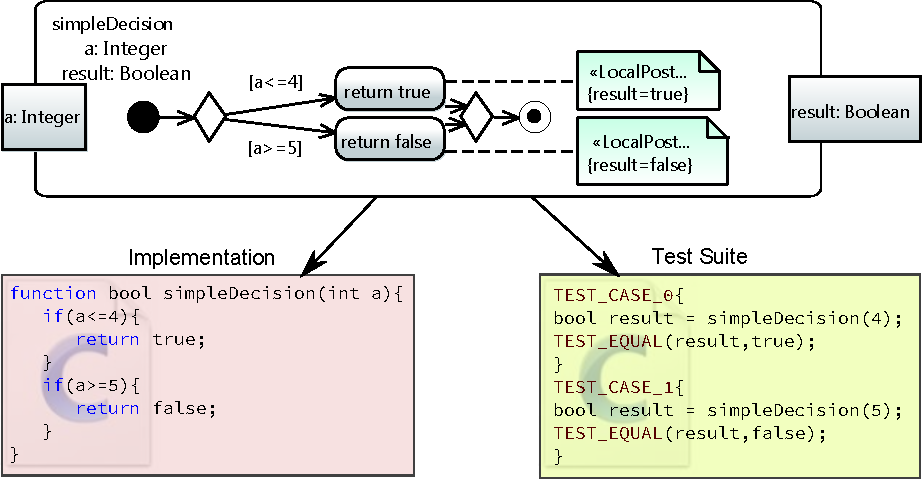
\includegraphics[width=\textwidth]{../Thesis/pics/BasicExamplesSimpleDecision.pdf}
\end{frame}
\subsection{Overview of our Solution}
\begin{frame}
\frametitle{Overview of our Solution}
\begin{description}
\item[Test Model:] A UML activity diagram with embedded OCL constraints modelling an operation/function is used as test model.
\item[Symbolic Execution:] Control flow paths within the activity diagram are executed and stored as constraint satisfaction problem.
\item[Constraint Solving:] A variety of state--of--the--art constraint solvers can be used to generate test data for an executed control flow path.
\item[Language Independent:] Test model and test cases and are stored as an instance of our own intermediate meta models.
\end{description}
\end{frame}


\section{The Algorithm}
\begin{frame}
\frametitle{Overview of the Algorithm}
\begin{block}{Normalisation}
Map UML/OCL to simplified intermediate representation
\end{block}
\begin{block}{Rigorous Mathematical Programming}
Transform activity diagram into an AMPL model
\end{block}
\begin{block}{Abstract Test Case Generation}
Find control flow paths using depth first and breadth first search
\end{block}
\begin{block}{Specific Test Data Generation}
Solve constraint satisfaction problem for each control flow path
\end{block}
\begin{block}{Unit Test Synthesis}
Output test cases as C++ unit tests using the boost test library
\end{block}
\end{frame}
\subsection{Normalisation}
\begin{frame}
\frametitle{The Activity Test Case Graph Model}
	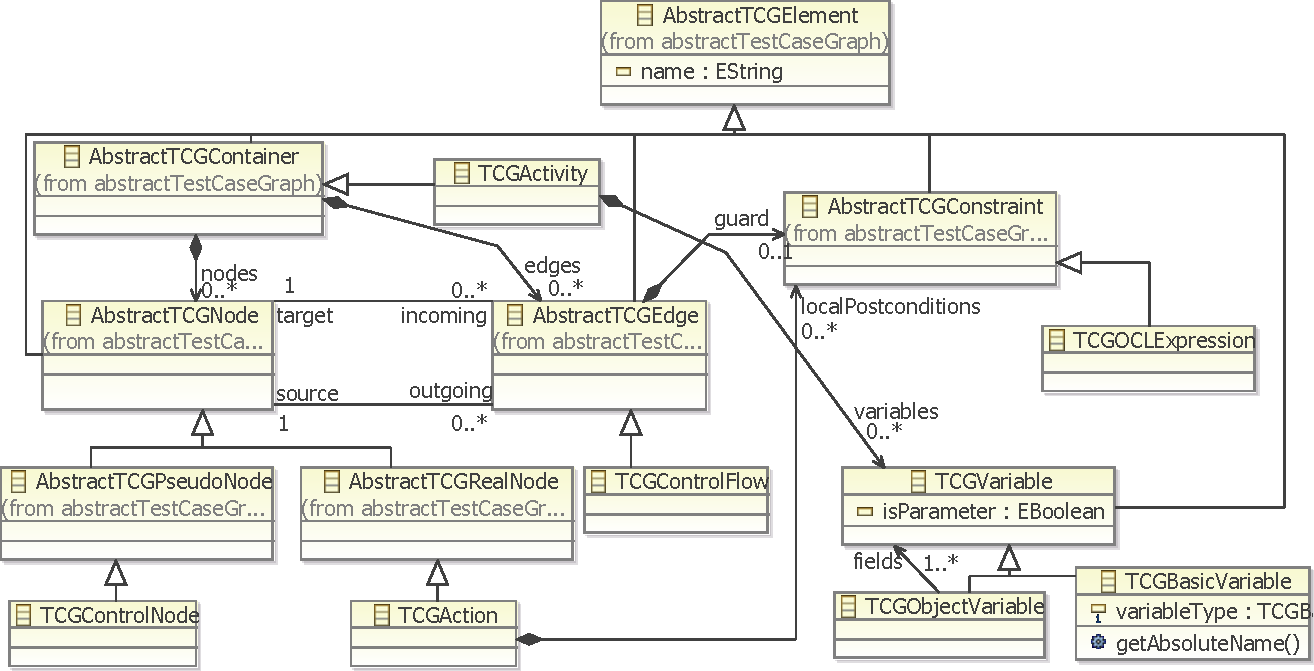
\includegraphics[width=\textwidth]{../IntermediatePresentation/pics/completeMetamodelforSlideshowN.pdf}
\end{frame}
\begin{frame}
\frametitle{Goals of Normalisation}
\begin{itemize}
  \item Ensure uniqueness of element names
  \item Slice relevant parts out of a huge UML model
  \item Parse embedded OCL constraints and ensure that they comply to the handled OCL subset
  \item Add continuity constraints 
\end{itemize}
\end{frame}

\subsection{AMPL Modelling}
\begin{frame}[fragile]
\frametitle{Introductory Example}
\begin{columns}
 \column{.39\textwidth} \ 
	\begin{block}{Activity Diagram} 
	\def\svgwidth{\textwidth}
	\scriptsize
	\import{pics/}{BasicExamples.pdf_tex}
	\end{block} 
\column{.56\textwidth} \ 
	\begin{block}{AMPL Model} 
		\begin{lstlisting}[basicstyle=\ttfamily\scriptsize,language=ampl]
param l; #Pathlength

# Variables (Property or Parameter)
var x{0..l} : integer := 1;
var y : integer := 1;

# Postconditions
set t within {0..l} default {};
s.t. t_post0{i in t} : (y)=(x[i-1]);
s.t. t_post1{i in t} : (x[i])=(x[i-1]);
set e within {0..l} default {};
s.t. e_post0{i in e} : (y)=(x[i-1]-100);
s.t. e_post0{i in e} : (x[i])=(x[i-1]);

# Guards
set d2e within {0..l} default {};
s.t. d2e_g{i in d2e} : (x[i])>=(6.0);
set d2t within {0..l} default {};
s.t. d2t_g{i in d2t} : (x[i])<=(5.0);
\end{lstlisting}
	\end{block} 
\end{columns}
\end{frame}

\begin{frame}[fragile]
\frametitle{Introductory Example}
	\begin{block}{Specify Path} 
		\begin{lstlisting}[basicstyle=\ttfamily\small,language=ampl]
param l := 1;
set d2f:= 0; # guard 
set f:= 1; # post condition
		\end{lstlisting}
	\end{block} 
	\begin{block}{Result} 
		\begin{lstlisting}[basicstyle=\ttfamily\small]
Solution determined by presolve.
a = 5
return = 0
		\end{lstlisting}
	\end{block}
\end{frame}

\begin{frame}
\frametitle{Slide Three} 
Body text / code of the frame goes here. 
\end{frame} 


\subsection{Subsection Name}

\begin{frame}
\frametitle{List Example One}
\begin{itemize} 
\item The first item.
\item The second item.
\item The third item.
\item The fourth item.
\end{itemize}
\end{frame}

\begin{frame}
\frametitle{List Example Two}
\begin{enumerate} 
\item The first item.
\item The second item.
\item The third item.
\item The fourth item.
\end{enumerate}
\end{frame}

\begin{frame}
\frametitle{List Example Three}
\begin{description}[Second Item] 
\item[First Item] Description of first item.
\item[Second Item] Description of second item.
\item[Third Item] Description of third item.
\item[Forth Item] Description of forth item.
\end{description}
\end{frame}

\section{Case Study}
\begin{frame}
\frametitle{Block Example One}
\begin{block}{Block Header}
	Block Body
\end{block}
\end{frame}

\begin{frame}
\frametitle{Block Example Two}
\begin{columns}
 \column{.45\textwidth} \ 
	\begin{block}{Block One Header} 
		Block One Body 
	\end{block} 
\column{.45\textwidth} \ 
	\begin{block}{Block Two Header} 
		Block Two Body
	\end{block} 
\end{columns}
\end{frame}

\end{document}
